% ─────────────────────────────────────────────────────────────────────────────
%  Informe: Simulador de Algoritmos de Reemplazo de Páginas
%  Asignatura: Sistemas Operativos
%  UNSAAC — Ingeniería Informática y Sistemas
% ─────────────────────────────────────────────────────────────────────────────
\documentclass[12pt, a4paper]{article}

% ── Paquetes ──────────────────────────────────────────────────────────────────
\usepackage[utf8]{inputenc}
\usepackage[T1]{fontenc}
\usepackage[spanish]{babel}
\usepackage{geometry}
\usepackage{graphicx}
\usepackage{float}
\usepackage{booktabs}
\usepackage{array}
\usepackage{tabularx}
\usepackage{longtable}
\usepackage{xcolor}
\usepackage{listings}
\usepackage{amsmath}
\usepackage{amssymb}
\usepackage{hyperref}
\usepackage{fancyhdr}
\usepackage{titlesec}
\usepackage{parskip}
\usepackage{enumitem}
\usepackage{caption}
\usepackage{subcaption}
\usepackage{tcolorbox}
\usepackage{mdframed}

\geometry{
  top=2.5cm, bottom=2.5cm,
  left=3cm,  right=2.5cm
}

% ── Colores ───────────────────────────────────────────────────────────────────
\definecolor{azulUNSAAC}{RGB}{0,70,127}
\definecolor{grisClaro}{RGB}{245,245,245}
\definecolor{rojoFallo}{RGB}{220,53,69}
\definecolor{verdeHit}{RGB}{40,167,69}
\definecolor{codigoFondo}{RGB}{248,248,248}
\definecolor{codigoBorde}{RGB}{200,200,200}

% ── Estilos de sección ────────────────────────────────────────────────────────
\titleformat{\section}
  {\large\bfseries\color{azulUNSAAC}}
  {\thesection.}{0.5em}{}[\titlerule]

\titleformat{\subsection}
  {\normalsize\bfseries\color{azulUNSAAC}}
  {\thesubsection.}{0.5em}{}

\titleformat{\subsubsection}
  {\normalsize\bfseries}
  {\thesubsubsection.}{0.5em}{}

% ── Cabecera y pie de página ──────────────────────────────────────────────────
\pagestyle{fancy}
\fancyhf{}
\fancyhead[L]{\small\textit{Simulador de Algoritmos de Reemplazo de Páginas}}
\fancyhead[R]{\small\textit{Sistemas Operativos — UNSAAC}}
\fancyfoot[C]{\thepage}
\renewcommand{\headrulewidth}{0.4pt}

% ── Configuración de listings (código) ───────────────────────────────────────
\lstset{
  backgroundcolor=\color{codigoFondo},
  basicstyle=\ttfamily\small,
  breaklines=true,
  frame=single,
  rulecolor=\color{codigoBorde},
  numbers=left,
  numberstyle=\tiny\color{gray},
  keywordstyle=\color{blue}\bfseries,
  commentstyle=\color{gray}\itshape,
  stringstyle=\color{teal},
  showstringspaces=false,
  tabsize=2,
}

% ── Cajas informativas ────────────────────────────────────────────────────────
\tcbuselibrary{skins, breakable}
\newtcolorbox{infobox}[1][]{
  colback=azulUNSAAC!5!white,
  colframe=azulUNSAAC!60!white,
  fonttitle=\bfseries,
  #1
}

% ─────────────────────────────────────────────────────────────────────────────
\begin{document}

% ── Portada ───────────────────────────────────────────────────────────────────
\begin{titlepage}
    \centering

    % Coloca el logo institucional en la misma carpeta que este archivo.
    % Descárgalo de: https://www.unsaac.edu.pe
    \includegraphics[width=0.22\textwidth]{logo.png}\\[0.6cm]

    {\Large\bfseries UNIVERSIDAD NACIONAL SAN ANTONIO ABAD DEL CUSCO\\}
    {\large\bfseries DEPARTAMENTO ACADÉMICO DE INFORMÁTICA\\}
    {\large\bfseries INGENIERÍA INFORMÁTICA Y SISTEMAS\\[1.2cm]}

    {\LARGE\bfseries SIMULADOR INTERACTIVO DE ALGORITMOS\\}
    {\LARGE\bfseries DE REEMPLAZO DE PÁGINAS\\[0.4cm]}
    {\Large\bfseries (Memoria Virtual y Gestión de Marcos)\\[1.2cm]}

    \begin{tabular}{@{}ll@{}}
        \textbf{ASIGNATURA:} & Sistemas Operativos \\
        \textbf{DOCENTE:}    & José Mauro Pillco \\
    \end{tabular}

    \vspace{1.0cm}

    \begin{minipage}{0.85\textwidth}
        \textbf{ALUMNO:}\\
        Bazarorda Cuellar, Héctor\\
    \end{minipage}

    \vfill

    {\large Cusco -- Perú\\}
    {\large 2025}
\end{titlepage}

% ── Tabla de contenidos ───────────────────────────────────────────────────────
\tableofcontents
\newpage

% ─────────────────────────────────────────────────────────────────────────────
\section{Introducción}
% ─────────────────────────────────────────────────────────────────────────────

La \textbf{memoria virtual} es una de las abstracciones fundamentales que proveen los sistemas operativos modernos. Permite que los procesos dispongan de un espacio de direcciones lógico que puede ser mucho mayor que la memoria física instalada en el sistema. El mecanismo subyacente es la \textbf{paginación}: el espacio de direcciones se divide en bloques de tamaño fijo llamados \emph{páginas}, y la memoria física se divide en bloques equivalentes llamados \emph{marcos} (\textit{frames}).

Cuando un proceso referencia una página que no se encuentra cargada en ningún marco físico, el hardware genera una \textbf{interrupción de fallo de página} (\textit{page fault}). El sistema operativo debe entonces decidir qué página desalojar para hacer espacio a la nueva. Esta decisión la toma el \textbf{algoritmo de reemplazo de páginas}, y su calidad impacta directamente en el rendimiento del sistema.

El presente trabajo describe el diseño, implementación y análisis de un \textbf{simulador interactivo paso a paso} que permite observar el comportamiento de siete algoritmos clásicos de reemplazo de páginas: FIFO, LRU, NRU, OPT, Clock, LFU y MFU. El simulador ha sido desarrollado como aplicación web con React~19, TypeScript y Tailwind~CSS, y ofrece visualización en tiempo real de estructuras internas, estadísticas de rendimiento y un panel de métricas detallado.

% ─────────────────────────────────────────────────────────────────────────────
\section{Marco Teórico}
% ─────────────────────────────────────────────────────────────────────────────

\subsection{Memoria Virtual y Paginación}

La memoria virtual desacopla las direcciones lógicas que usa un proceso de las direcciones físicas de la RAM. Una \textbf{tabla de páginas} almacena la correspondencia entre número de página lógica y número de marco físico. Cuando el bit de presencia de una entrada es~0, la página reside en disco y cualquier acceso genera un \textit{page fault}.

\subsection{Fallo de Página}

Secuencia de eventos ante un fallo de página:
\begin{enumerate}
  \item La MMU detecta la ausencia de la página y genera una excepción (\textit{trap}).
  \item El SO toma el control, busca la página en el área de \textit{swap} del disco.
  \item Si existen marcos libres, carga la página en uno de ellos.
  \item Si \textbf{no} hay marcos libres, se ejecuta el \textbf{algoritmo de reemplazo} para elegir la víctima.
  \item La página víctima se guarda en disco (si su bit~M está activo) y la nueva página se carga.
  \item Se actualiza la tabla de páginas y se retoma la ejecución del proceso.
\end{enumerate}

Cada fallo genera al menos una \textbf{llamada al sistema} (la excepción en sí) y una \textbf{lectura de disco}, haciendo que los fallos sean órdenes de magnitud más costosos que los aciertos.

\subsection{Anomalía de Bélady}

Para la mayoría de los algoritmos, aumentar el número de marcos reduce los fallos. Sin embargo, en FIFO existe la posibilidad de que agregar más marcos \emph{incremente} el número de fallos. Este fenómeno se denomina \textbf{Anomalía de Bélady} y se ilustra con la secuencia clásica 1-2-3-4-1-2-5-1-2-3-4-5:

\begin{center}
\begin{tabular}{lcc}
  \toprule
  Algoritmo & 3 marcos & 4 marcos \\
  \midrule
  FIFO & 9 fallos & 10 fallos \textcolor{rojoFallo}{(+1)} \\
  OPT  & 8 fallos &  6 fallos \textcolor{verdeHit}{(-2)} \\
  \bottomrule
\end{tabular}
\end{center}

% ─────────────────────────────────────────────────────────────────────────────
\section{Algoritmos de Reemplazo de Páginas}
% ─────────────────────────────────────────────────────────────────────────────

\subsection{FIFO — First In, First Out}

\subsubsection{Descripción}

FIFO es el algoritmo más simple. Mantiene una \textbf{cola circular} de páginas ordenada por orden de llegada. Al producirse un fallo con memoria llena, expulsa la página que lleva más tiempo residente en memoria, independientemente de si fue usada recientemente.

\subsubsection{Funcionamiento}

\begin{itemize}
  \item Se mantiene un puntero \texttt{fifoPointer} sobre los marcos.
  \item Ante un fallo, la víctima es el marco al que apunta el puntero; luego el puntero avanza en módulo \(n\) (número de marcos).
  \item Los hits no modifican ni el puntero ni el orden de la cola.
\end{itemize}

\subsubsection{Análisis con secuencia ejemplo}

Secuencia: \(1,2,3,4,1,2,5,1,2,3,4,5\) — 4 marcos:

\begin{center}
\small
\begin{tabular}{ccccccccccccc}
  \toprule
  Paso  & 1 & 2 & 3 & 4 & 5 & 6 & 7 & 8 & 9 & 10 & 11 & 12 \\
  Pág.  & 1 & 2 & 3 & 4 & 1 & 2 & 5 & 1 & 2 & 3  & 4  & 5  \\
  \midrule
  F0 & \textbf{1} & 1 & 1 & 1 & 1 & 1 & \textbf{5} & 5 & 5 & 5  & \textbf{4}  & 4  \\
  F1 & -- & \textbf{2} & 2 & 2 & 2 & 2 & 2 & \textbf{1} & 1 & 1  & 1   & \textbf{5}  \\
  F2 & -- & -- & \textbf{3} & 3 & 3 & 3 & 3 & 3 & \textbf{2} & 2  & 2   & 2  \\
  F3 & -- & -- & -- & \textbf{4} & 4 & 4 & 4 & 4 & 4 & \textbf{3}  & 3   & 3  \\
  \midrule
  Fallo & F & F & F & F & -- & -- & F & F & F & F  & F  & F  \\
  \bottomrule
\end{tabular}
\end{center}

\textbf{Total fallos: 10} de 12 referencias (83.3\%). Eficiencia vs OPT: 60\%.

\subsubsection{Ventajas y desventajas}

\begin{infobox}[title={FIFO}]
\textbf{Ventaja:} Implementación trivial (un puntero entero). \\
\textbf{Desventaja:} No considera la frecuencia ni la recencia de uso. Sufre la \textit{Anomalía de Bélady}.
\end{infobox}

% ──────────────────────────────────────────────────
\subsection{LRU — Least Recently Used}

\subsubsection{Descripción}

LRU expulsa la página que no ha sido accedida por más tiempo. Se basa en el \textbf{principio de localidad temporal}: si una página se usó recientemente, probablemente se vuelva a usar pronto.

\subsubsection{Funcionamiento}

\begin{itemize}
  \item Cada marco almacena un \textbf{timestamp} (\texttt{lastUsed}) que se actualiza en cada acceso.
  \item Ante un fallo, se expulsa el marco con el timestamp más pequeño (el más antiguo).
  \item Los hits también actualizan el timestamp del marco correspondiente.
\end{itemize}

\subsubsection{Análisis}

Con la misma secuencia y 4 marcos, LRU produce \textbf{8 fallos} (66.7\%), mejorando a FIFO por 2 fallos.

\subsubsection{Ventajas y desventajas}

\begin{infobox}[title={LRU}]
\textbf{Ventaja:} Buena aproximación al óptimo en cargas reales con localidad temporal. \\
\textbf{Desventaja:} En hardware puro requiere hardware de seguimiento (costoso). En la práctica se usan aproximaciones (Clock, NFU).
\end{infobox}

% ──────────────────────────────────────────────────
\subsection{NRU — Not Recently Used}

\subsubsection{Descripción}

NRU clasifica las páginas en cuatro clases según dos bits de estado:
\begin{itemize}
  \item \textbf{Bit R} (Referenced): se pone a~1 al acceder a la página. Se resetea periódicamente por el SO.
  \item \textbf{Bit M} (Modified / Dirty): se pone a~1 si la página fue modificada (escritura).
\end{itemize}

\begin{center}
\begin{tabular}{cccc}
  \toprule
  Clase & R & M & Prioridad de reemplazo \\
  \midrule
  C0 & 0 & 0 & Más alta (primera candidata) \\
  C1 & 0 & 1 & Segunda \\
  C2 & 1 & 0 & Tercera \\
  C3 & 1 & 1 & Más baja (última candidata) \\
  \bottomrule
\end{tabular}
\end{center}

\subsubsection{Funcionamiento}

\begin{enumerate}
  \item En cada acceso, el bit~R del marco se activa.
  \item Cada \texttt{RESET\_INTERVAL}~$= 4$ pasos, el SO resetea todos los bits~R (simula el tick del temporizador).
  \item Ante un fallo, se selecciona el primer frame de la clase más baja disponible.
\end{enumerate}

El bit~M se inicializa con una función determinista sobre el número de página, pero puede sobreescribirse manualmente en el simulador haciendo clic sobre el badge \texttt{M=0}/\texttt{M=1} en la tabla de marcos.

\subsubsection{Ventajas y desventajas}

\begin{infobox}[title={NRU}]
\textbf{Ventaja:} Fácil de implementar en hardware con dos bits. Diferencia entre páginas limpias y sucias (evitar escrituras a disco innecesarias). \\
\textbf{Desventaja:} Clasificación gruesa (solo 4 clases); puede expulsar páginas no óptimas dentro de una misma clase.
\end{infobox}

% ──────────────────────────────────────────────────
\subsection{OPT — Algoritmo Óptimo de Bélady}

\subsubsection{Descripción}

OPT (también llamado MIN o algoritmo de Bélady) reemplaza la página cuyo \textbf{próximo uso sea más lejano en el futuro}, o la que nunca volverá a usarse. Produce el número mínimo posible de fallos para cualquier secuencia y número de marcos dados, siendo la referencia teórica ideal.

\subsubsection{Funcionamiento}

\begin{enumerate}
  \item Para cada página en memoria, se busca en el resto de la secuencia cuándo ocurre su próximo acceso.
  \item La página con mayor distancia al próximo uso (o \(\infty\) si nunca se usa) es la víctima.
  \item \textbf{Desempate}: si varias páginas tienen el mismo próximo uso, se expulsa la que llegó primero a memoria (criterio FIFO sobre \texttt{arrivalOrder}), haciendo el algoritmo determinista.
\end{enumerate}

\subsubsection{Análisis}

Con la secuencia ejemplo y 4 marcos, OPT produce \textbf{6 fallos} (50\%), el mínimo teórico posible. Esta cifra sirve como denominador de la eficiencia de los demás algoritmos.

\subsubsection{Ventajas y desventajas}

\begin{infobox}[title={OPT}]
\textbf{Ventaja:} Mínimo número de fallos garantizado. Útil como referencia. \\
\textbf{Desventaja:} \textbf{No implementable} en un SO real (requiere conocer el futuro). Solo viable en simulaciones o en sistemas con trazas pregrabadas.
\end{infobox}

% ──────────────────────────────────────────────────
\subsection{Clock — Segunda Oportunidad}

\subsubsection{Descripción}

Clock es una aproximación eficiente a LRU que usa \textbf{un único bit de referencia} por frame y un puntero circular. Cuando una página es accedida, su bit se pone a~1. Al necesitar reemplazar, el puntero avanza buscando un frame con bit~$= 0$; los frames con bit~$= 1$ reciben una «segunda oportunidad» (su bit se resetea a~0 y el puntero sigue avanzando).

\subsubsection{Funcionamiento}

\begin{enumerate}
  \item \textbf{Hit}: se activa el \texttt{clockBit} del frame, el puntero no se mueve.
  \item \textbf{Fallo con frame libre}: se carga la página, el puntero avanza al siguiente.
  \item \textbf{Fallo sin frames libres}:
    \begin{itemize}
      \item Si \texttt{clockBit[pointer] = 1} → se pone a~0, el puntero avanza (\textit{second chance}).
      \item Si \texttt{clockBit[pointer] = 0} → esa página es reemplazada; el puntero avanza.
    \end{itemize}
  \item Se registra cuántos pasos dio el puntero (\texttt{stepsToReplace}).
\end{enumerate}

\subsubsection{Ventajas y desventajas}

\begin{infobox}[title={Clock}]
\textbf{Ventaja:} Implementación eficiente ($O(n)$ en el peor caso, $O(1)$ promedio). Páginas recién usadas no son expulsadas inmediatamente. \\
\textbf{Desventaja:} Puede no distinguir bien entre páginas de uso intermedio si todos los bits están en~1 (degenera a FIFO).
\end{infobox}

% ──────────────────────────────────────────────────
\subsection{LFU — Least Frequently Used}

\subsubsection{Descripción}

LFU reemplaza la página con la \textbf{menor frecuencia de acceso} acumulada. La idea es que las páginas muy usadas tienen mayor probabilidad de volver a usarse.

\subsubsection{Funcionamiento}

\begin{itemize}
  \item Cada frame mantiene un contador \texttt{frequency} que se incrementa en cada acceso (hit o carga inicial).
  \item Ante un fallo, se expulsa el frame con menor \texttt{frequency}.
  \item \textbf{Desempate}: si dos frames tienen igual frecuencia, se expulsa el menos recientemente usado (LRU sobre \texttt{lastUsed}).
  \item Al cargar una página nueva, su \texttt{frequency} se inicializa en~1.
\end{itemize}

\subsubsection{Ventajas y desventajas}

\begin{infobox}[title={LFU}]
\textbf{Ventaja:} Páginas muy usadas permanecen en memoria. \\
\textbf{Desventaja:} Una página intensamente usada en el pasado pero ya innecesaria puede «contaminar» el cache por su alto contador, retrasando su evicción.
\end{infobox}

% ──────────────────────────────────────────────────
\subsection{MFU — Most Frequently Used}

\subsubsection{Descripción}

MFU es el algoritmo inverso a LFU: reemplaza la página con la \textbf{mayor frecuencia de acceso}. La hipótesis es que las páginas con alta frecuencia ya han sido suficientemente servidas, mientras que las páginas de baja frecuencia son recientes y probablemente se necesitarán pronto.

\subsubsection{Funcionamiento}

Idéntico a LFU salvo que la selección de víctima busca el \textbf{máximo} de \texttt{frequency} en lugar del mínimo. El desempate también usa LRU sobre \texttt{lastUsed}.

\subsubsection{Ventajas y desventajas}

\begin{infobox}[title={MFU}]
\textbf{Ventaja:} Útil en patrones donde las páginas de uso intensivo son temporales (ráfagas cortas). \\
\textbf{Desventaja:} En la mayoría de cargas reales produce más fallos que LFU y LRU; es fundamentalmente un algoritmo didáctico.
\end{infobox}

% ─────────────────────────────────────────────────────────────────────────────
\section{Descripción del Simulador}
% ─────────────────────────────────────────────────────────────────────────────

\subsection{Objetivo}

El simulador tiene como objetivo permitir la visualización interactiva del comportamiento paso a paso de los siete algoritmos anteriores, mostrando en cada momento:
\begin{itemize}
  \item El estado completo de los marcos físicos.
  \item Las variables internas del algoritmo activo.
  \item Las estadísticas acumuladas (fallos, hits, eficiencia vs OPT).
  \item Un panel de métricas con información sobre recursos, tiempo, syscalls e interrupciones.
\end{itemize}

\subsection{Tecnologías Utilizadas}

\begin{center}
\begin{tabular}{ll}
  \toprule
  Tecnología & Rol \\
  \midrule
  React 19 + TypeScript & Interfaz declarativa y tipado estático \\
  Vite & Servidor de desarrollo y bundler \\
  Tailwind CSS v4 & Estilos utilitarios \\
  Framer Motion & Animaciones de celdas \\
  Vercel Analytics & Métricas de uso en producción \\
  \bottomrule
\end{tabular}
\end{center}

\subsection{Arquitectura}

El diseño sigue un patrón \textbf{pre-cómputo + navegación por índice}. Al ejecutar la simulación se genera un arreglo de \texttt{Snapshot[]} (uno por paso). La navegación entre pasos solo modifica un entero (\texttt{currentStep}), sin recalcular nada:

\begin{lstlisting}[language=,caption={Estructura de archivos del proyecto}]
src/
|-- types/index.ts           # FrameState, Snapshot, SimulatorState,
|                            # SimulationMetrics, AlgorithmVariables
|-- algorithms/
|   |-- fifo.ts   runFIFO(sequence, frameCount)
|   |-- lru.ts    runLRU(sequence, frameCount)
|   |-- nru.ts    runNRU(sequence, frameCount, dirtyOverrides)
|   |-- opt.ts    runOPT(sequence, frameCount)
|   |-- clock.ts  runClock(sequence, frameCount)
|   |-- lfu.ts    runLFU(sequence, frameCount)
|   |-- mfu.ts    runMFU(sequence, frameCount)
|   `-- utils.ts  emptyFrame(), cloneFrames()
|-- store/
|   `-- simulatorStore.tsx   useReducer + Context +
|                            computeSnapshots() + computeMetrics()
`-- components/
    |-- ConfigPanel.tsx      Configuracion del simulador
    |-- FrameTable.tsx       Tabla principal de marcos
    |-- StepControls.tsx     Navegacion y reproduccion
    |-- VariablesPanel.tsx   Variables internas del algoritmo
    |-- StatsPanel.tsx       Estadisticas y eficiencia
    `-- MetricsPanel.tsx     Metricas detalladas
\end{lstlisting}

\subsubsection{Flujo de datos}

\begin{enumerate}
  \item El usuario configura algoritmo, secuencia y número de marcos en \texttt{ConfigPanel}.
  \item Al pulsar \textit{Ejecutar}, se despacha la acción \texttt{RUN\_SIMULATION}.
  \item El reducer llama a \texttt{computeSnapshots()} → genera \texttt{Snapshot[]}.
  \item Inmediatamente llama a \texttt{computeMetrics()} → genera \texttt{SimulationMetrics}.
  \item Los componentes de visualización leen del estado global a través del hook \texttt{useSimulator()}.
\end{enumerate}

% ─────────────────────────────────────────────────────────────────────────────
\section{Funcionalidades del Simulador}
% ─────────────────────────────────────────────────────────────────────────────

\subsection{Panel de Configuración}

El panel izquierdo permite seleccionar el algoritmo, ingresar la secuencia de páginas y ajustar el número de marcos (1--20). Muestra los 7 algoritmos disponibles con su nombre y descripción breve.

\begin{figure}[H]
  \centering
  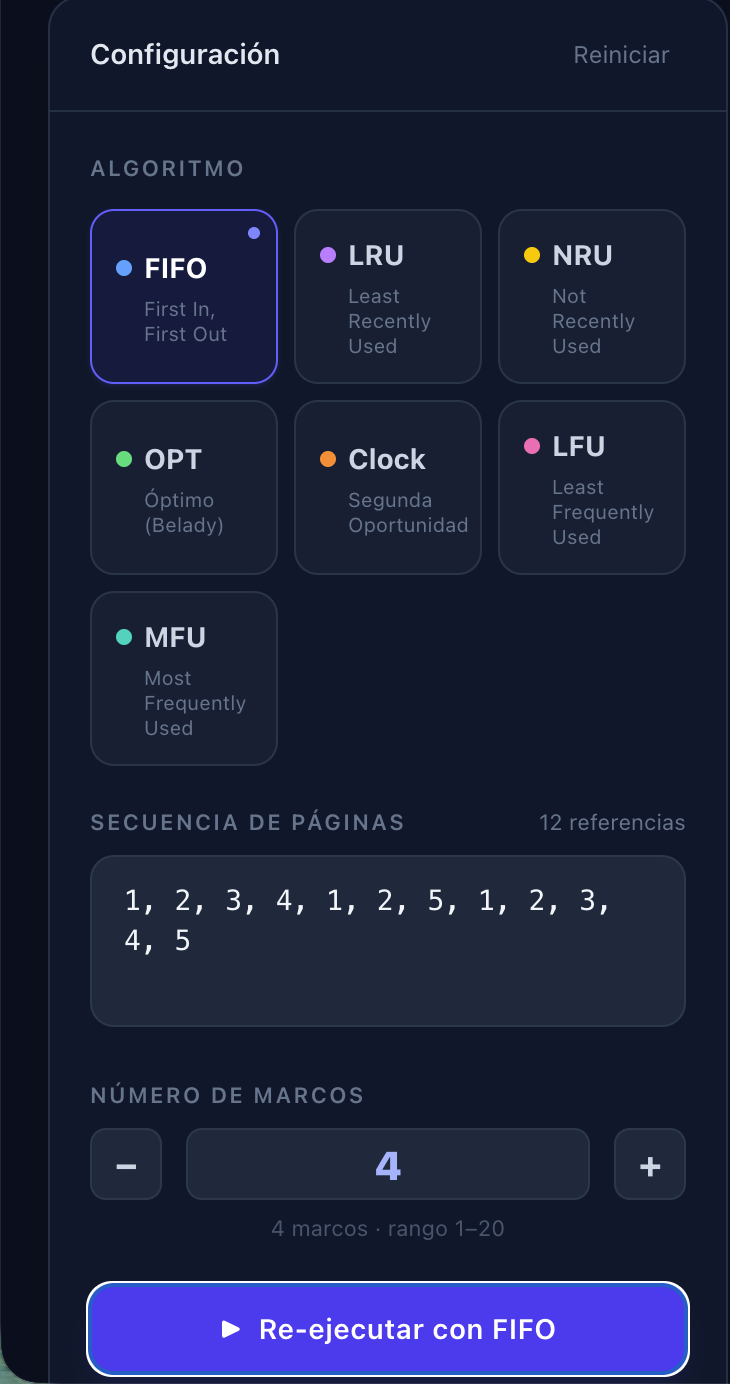
\includegraphics[width=0.45\textwidth]{cap1.png}
  \caption{Panel de configuración: selector de algoritmo, secuencia y número de marcos.}
  \label{fig:config}
\end{figure}

\subsection{Tabla de Marcos}

La tabla es el componente central del simulador. Las \textbf{filas} representan los marcos físicos y las \textbf{columnas} los pasos de tiempo de la secuencia.

\begin{figure}[H]
  \centering
  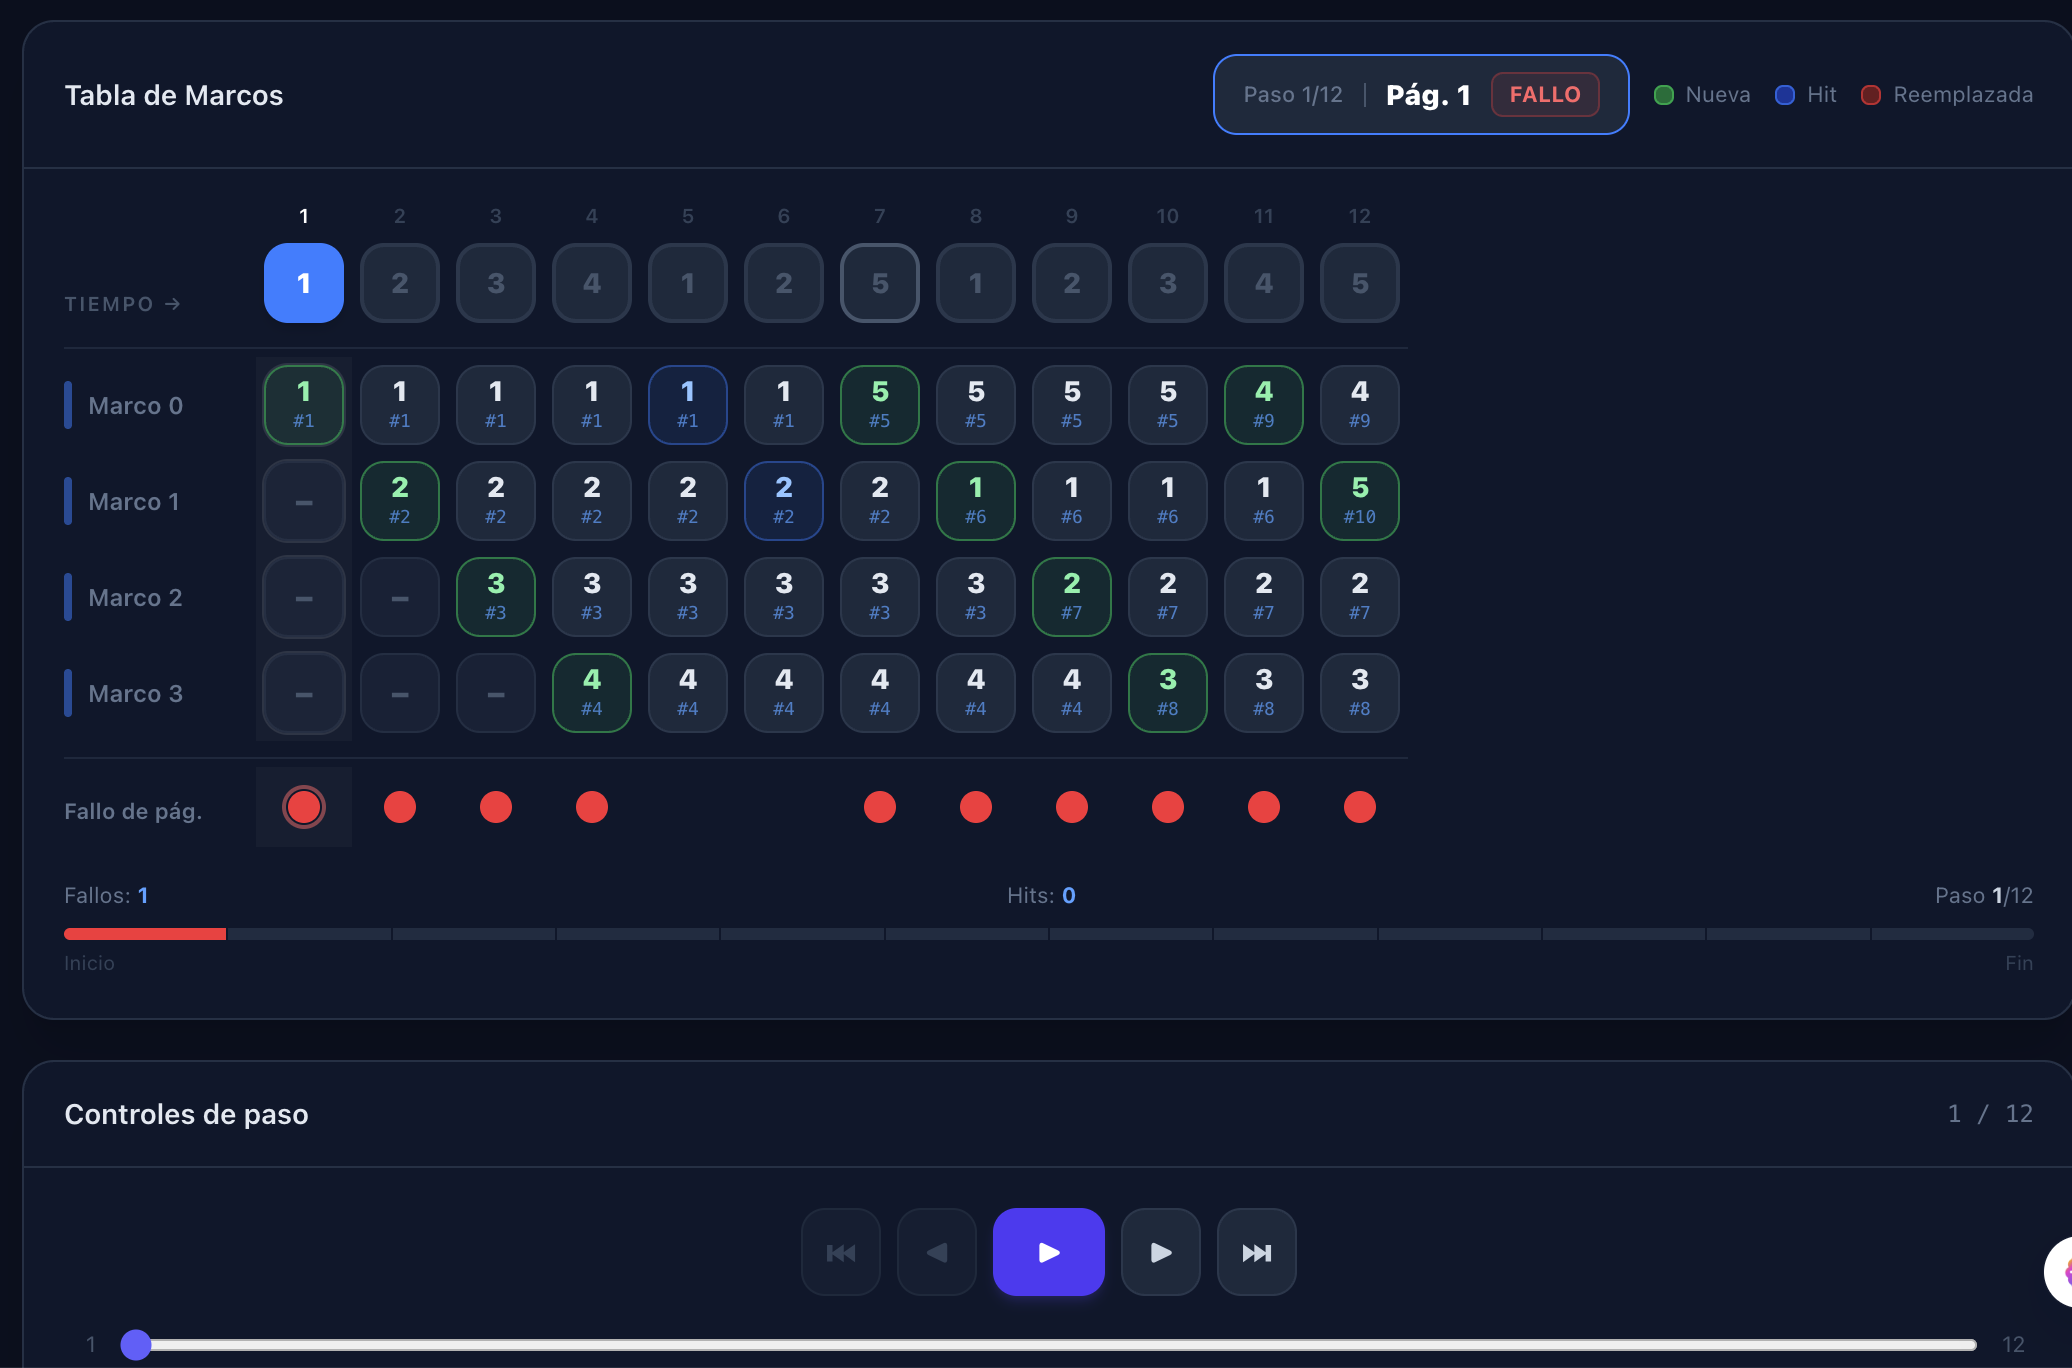
\includegraphics[width=\textwidth]{cap3.png}
  \caption{Tabla de marcos con FIFO — secuencia 1,2,3,4,1,2,5,1,2,3,4,5 con 4 marcos. Se muestran los indicadores de fallo de página (puntos rojos) en la fila inferior.}
  \label{fig:tabla}
\end{figure}

Código de colores de las celdas:
\begin{itemize}
  \item \textcolor{verdeHit}{\textbf{Verde}} — Página recién cargada en un frame vacío (\textit{load}).
  \item \textcolor{blue}{\textbf{Azul}} — Acceso con acierto (\textit{hit}).
  \item \textcolor{rojoFallo}{\textbf{Rojo}} — Página reemplazada (evicción).
  \item \textbf{Gris} — Frame ocupado sin cambios en este paso.
\end{itemize}

Cada celda muestra datos internos del algoritmo activo: orden de llegada en FIFO, timestamp en LRU, bits R/M y clase en NRU, bit de reloj en Clock, frecuencia en LFU/MFU.

\subsection{Panel de Variables Internas}

Muestra en tiempo real las estructuras internas del algoritmo en el paso actual. Por ejemplo, para FIFO se muestra el puntero y la cola ordenada por llegada:

\begin{figure}[H]
  \centering
  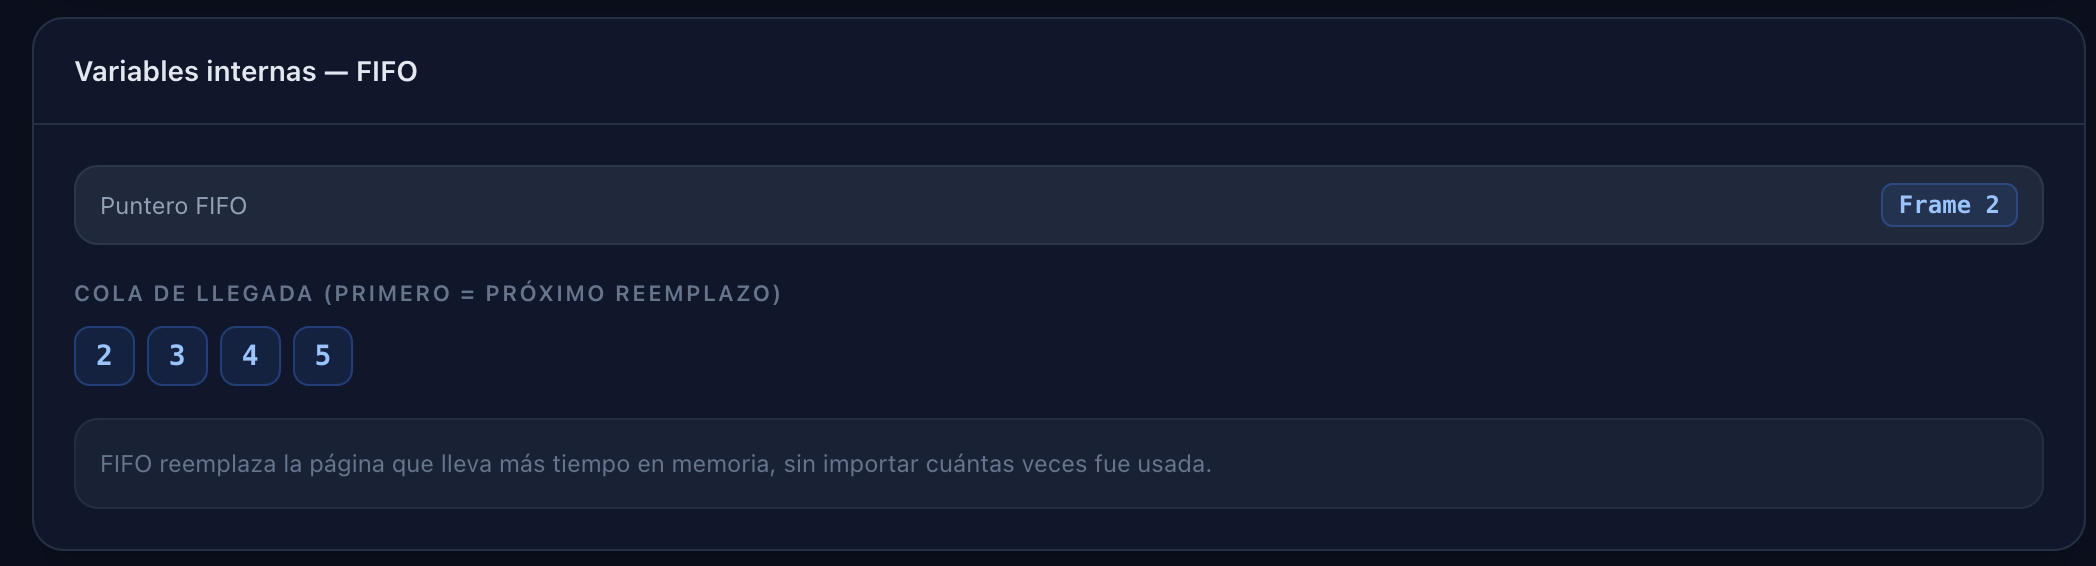
\includegraphics[width=\textwidth]{cap4.png}
  \caption{Variables internas de FIFO: puntero apuntando al Frame~2 y cola de páginas \{2, 3, 4, 5\} ordenada por llegada.}
  \label{fig:variables}
\end{figure}

\subsection{Vista con LRU}

\begin{figure}[H]
  \centering
  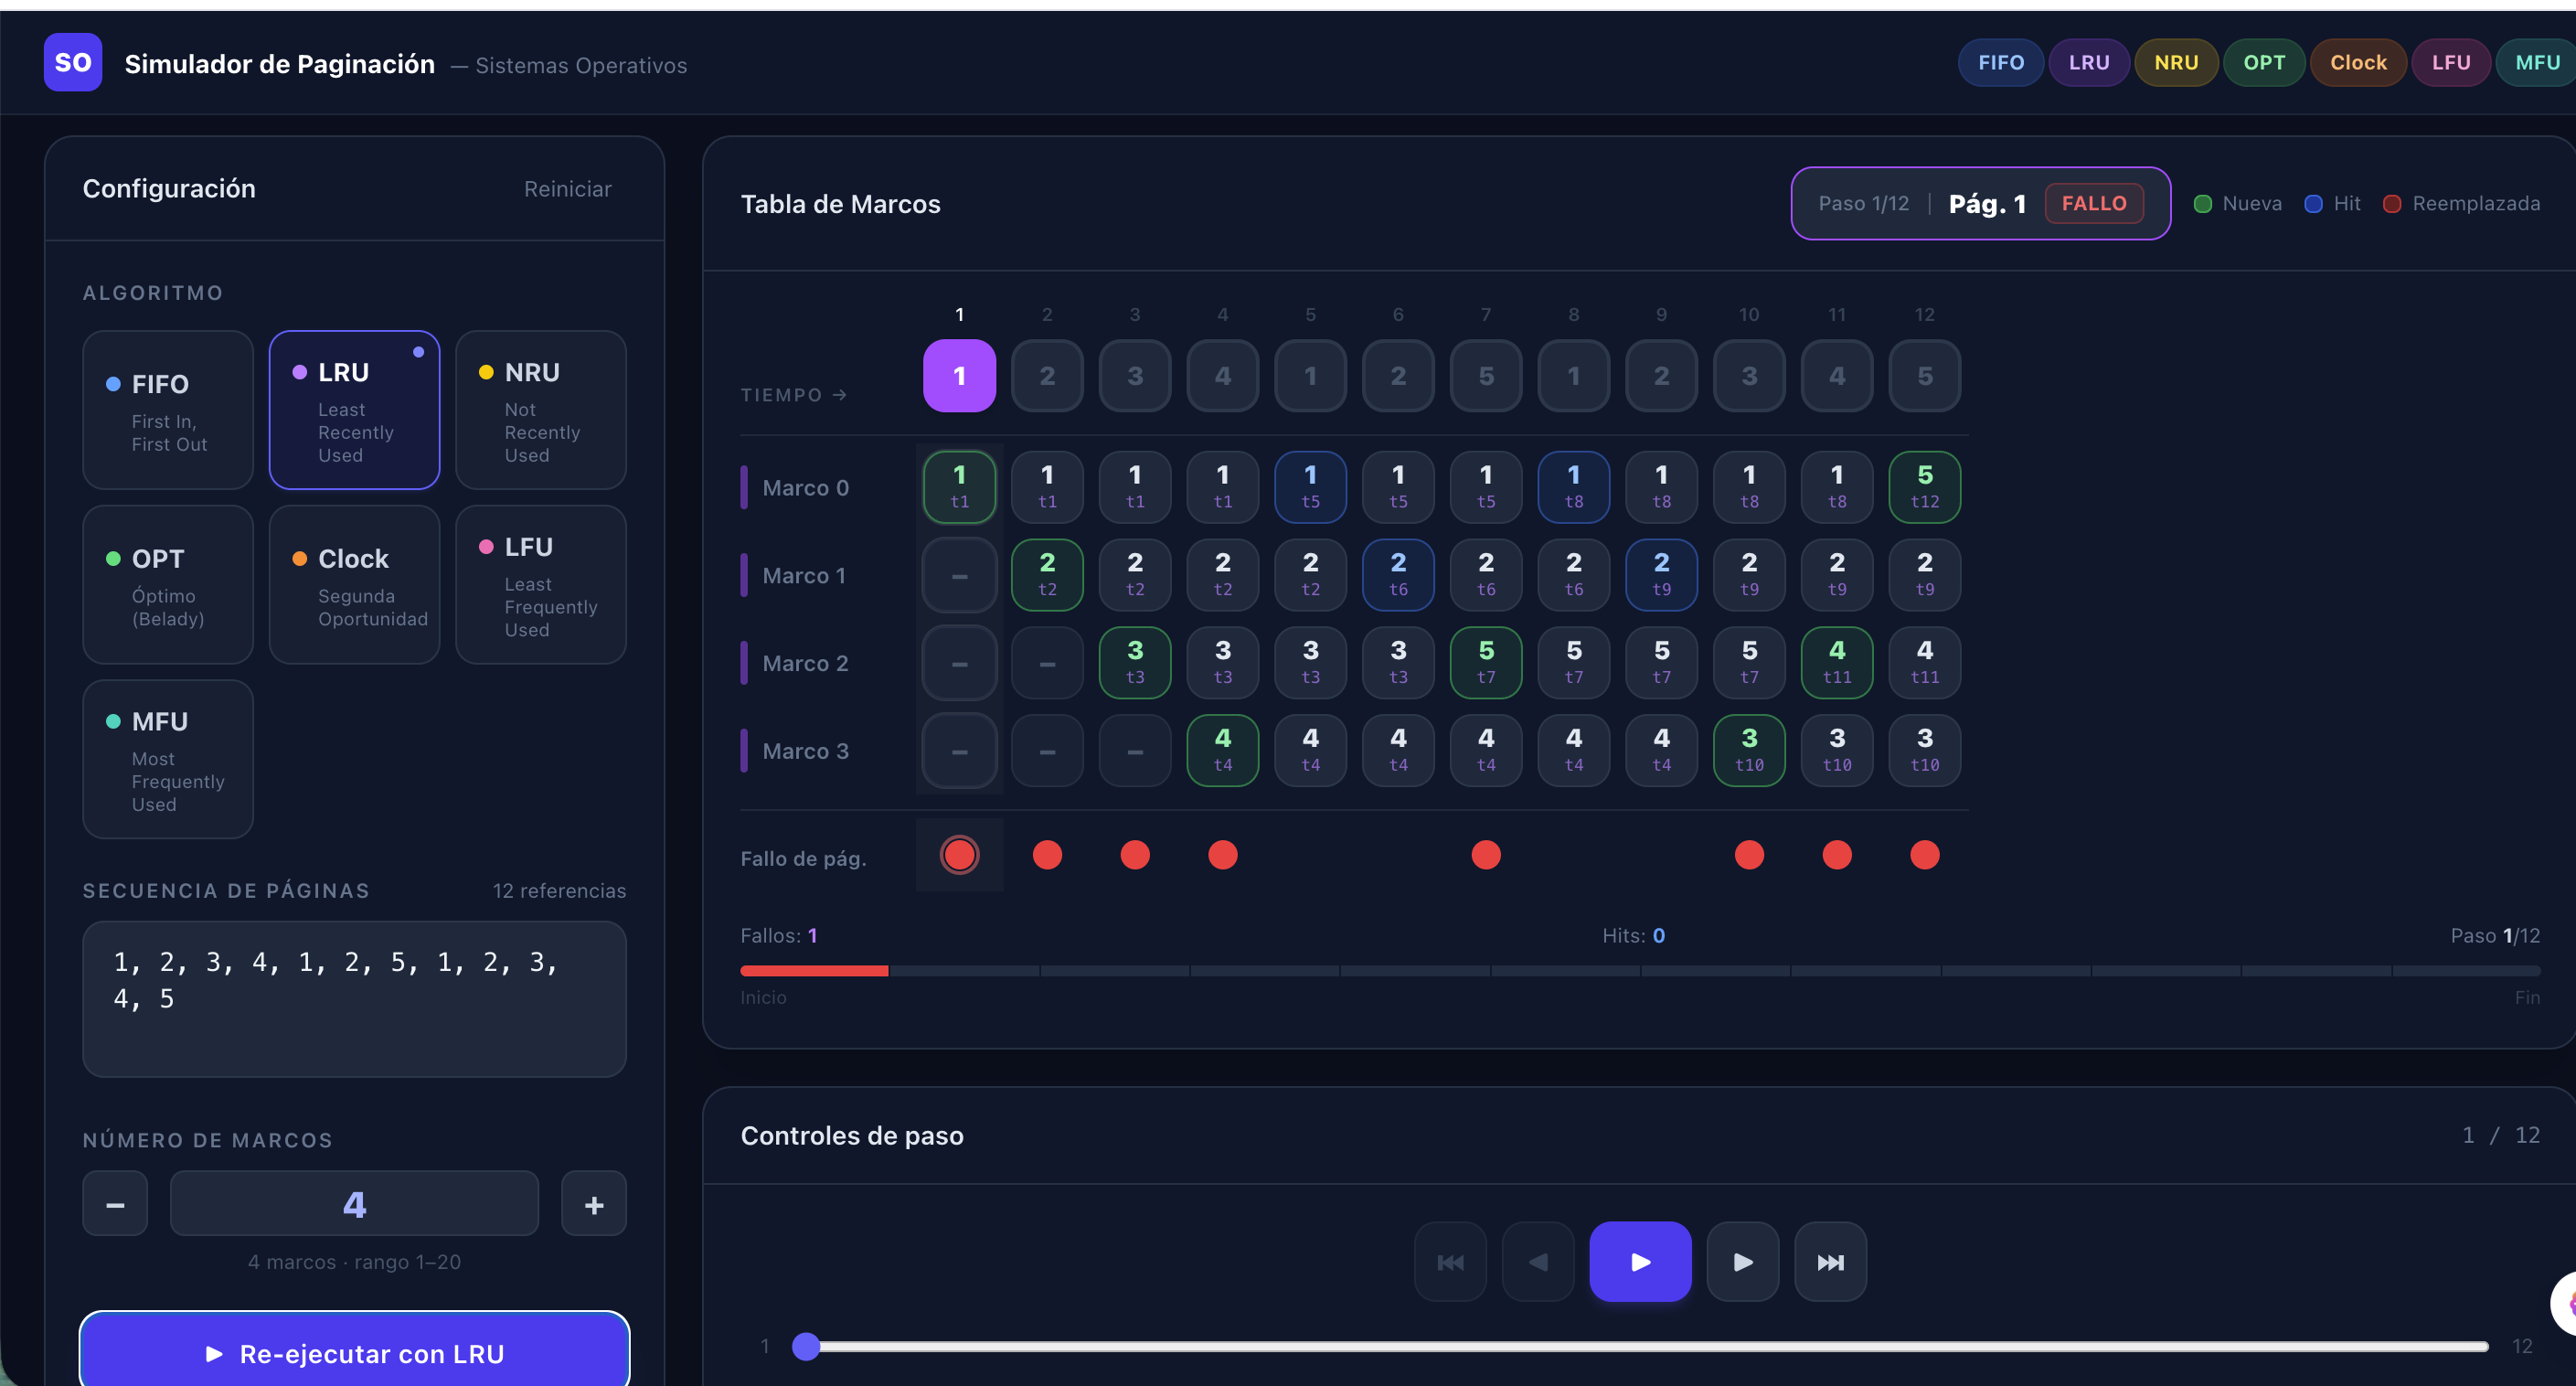
\includegraphics[width=\textwidth]{cap6.png}
  \caption{Vista completa del simulador con LRU seleccionado. Se aprecia la tabla de marcos y el botón de re-ejecución.}
  \label{fig:lru}
\end{figure}

\subsection{Vista con Clock}

\begin{figure}[H]
  \centering
  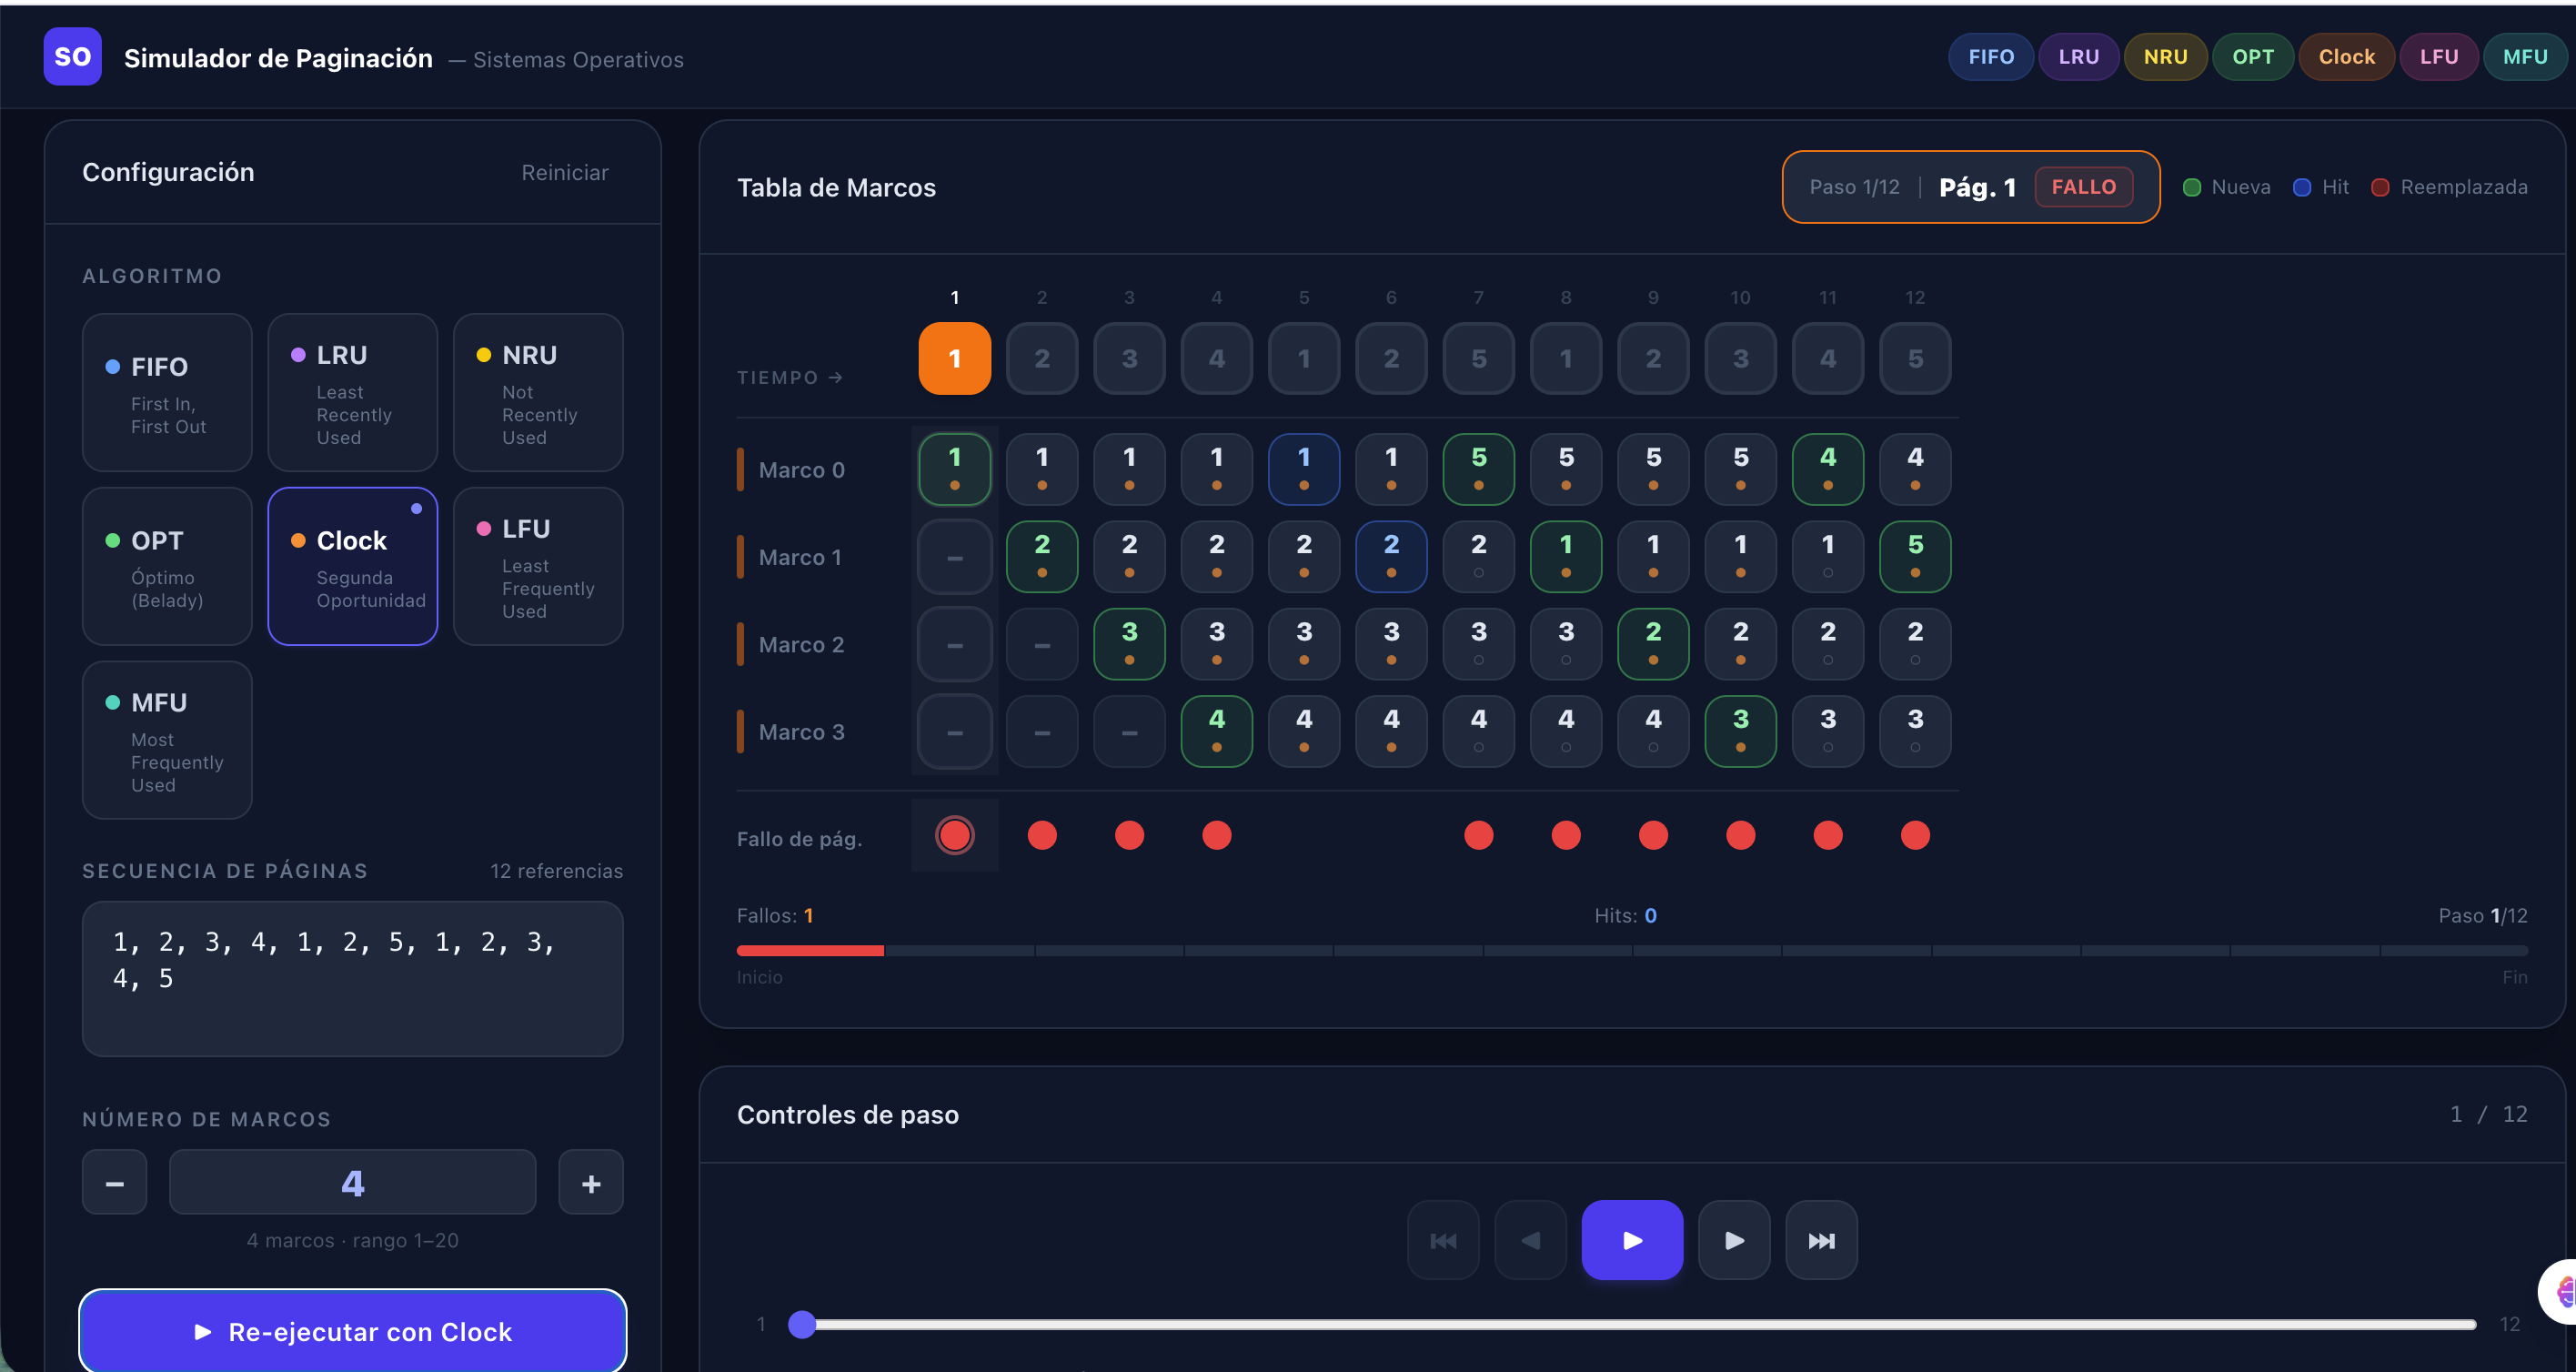
\includegraphics[width=\textwidth]{cap7.png}
  \caption{Simulación con el algoritmo Clock (Segunda Oportunidad). El bit de referencia circular se visualiza en cada celda.}
  \label{fig:clock}
\end{figure}

\subsection{Vista con NRU}

\begin{figure}[H]
  \centering
  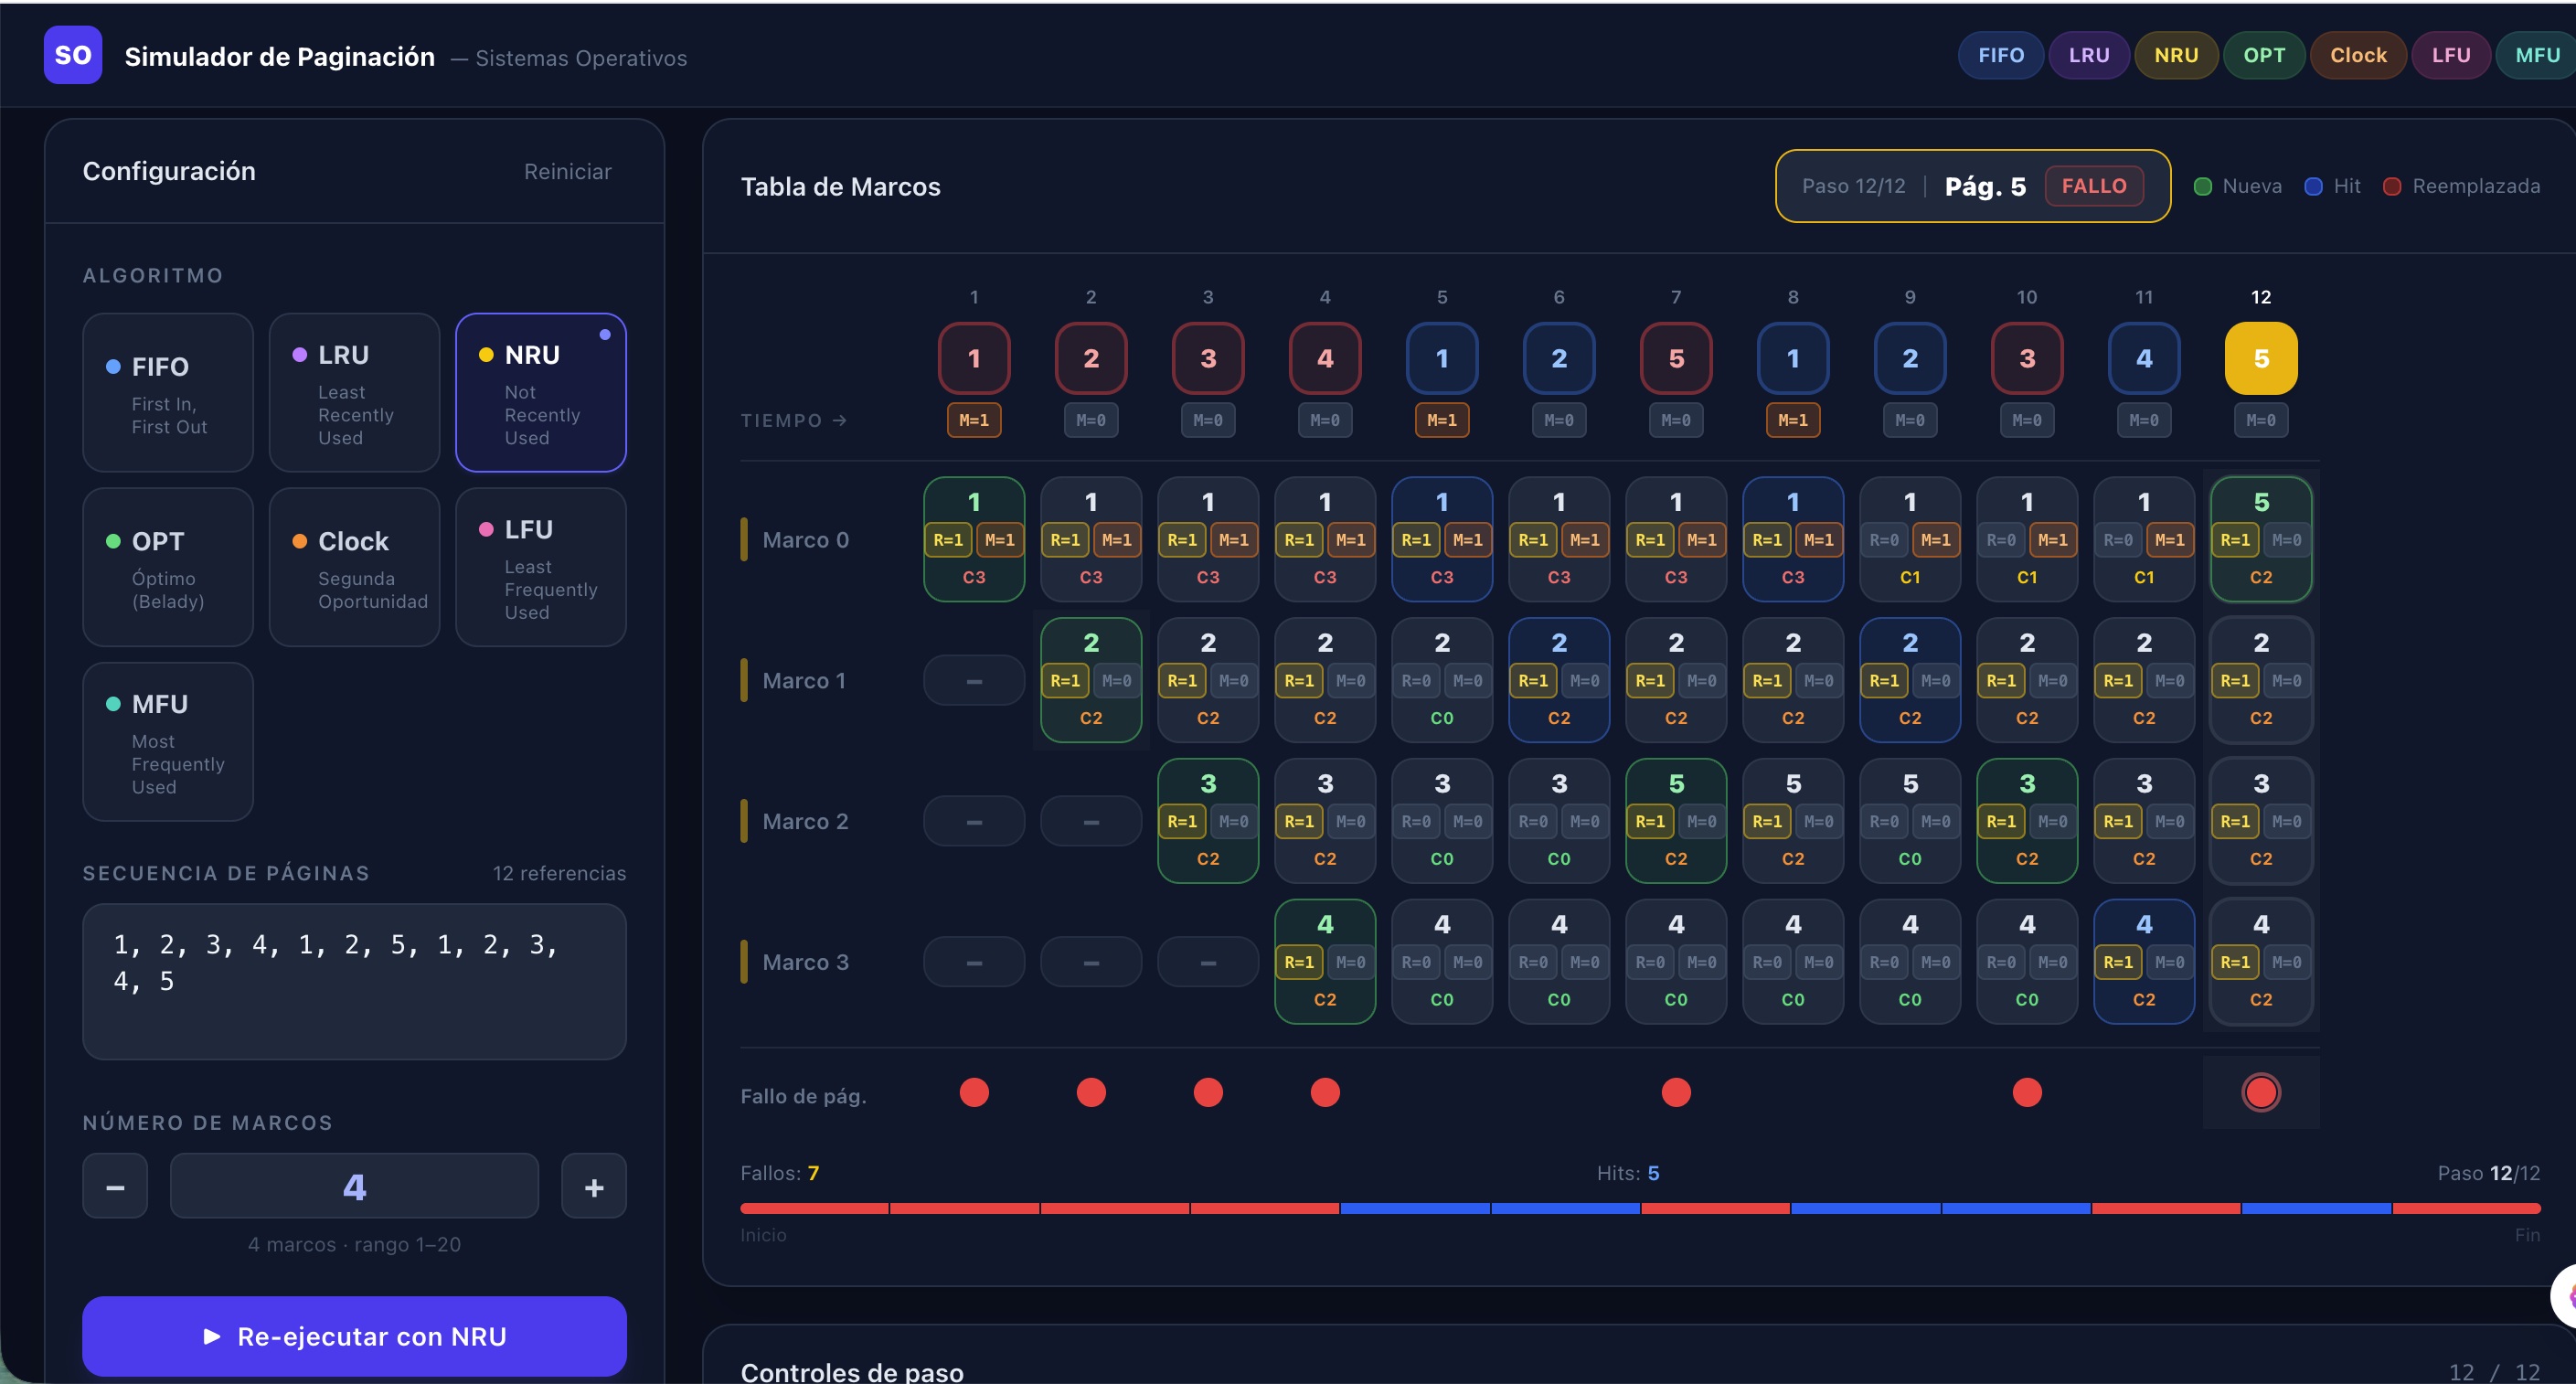
\includegraphics[width=\textwidth]{cap8.png}
  \caption{Simulación con NRU en el paso 5. Se muestran los bits R/M y la clase NRU asignada a cada frame. El badge M es editable con clic.}
  \label{fig:nru}
\end{figure}

\subsection{Controles de Navegación}

El componente \texttt{StepControls} ofrece:
\begin{itemize}
  \item Botones \textbf{anterior/siguiente}, \textbf{inicio/fin}.
  \item \textbf{Scrubber} (barra deslizante) para saltar a cualquier paso.
  \item \textbf{Reproducción automática} a 0.5×, 1×, 2× y 4× de velocidad.
\end{itemize}

% ─────────────────────────────────────────────────────────────────────────────
\section{Panel de Estadísticas}
% ─────────────────────────────────────────────────────────────────────────────

El panel de estadísticas muestra en tiempo real (actualizado en cada paso de navegación):

\begin{figure}[H]
  \centering
  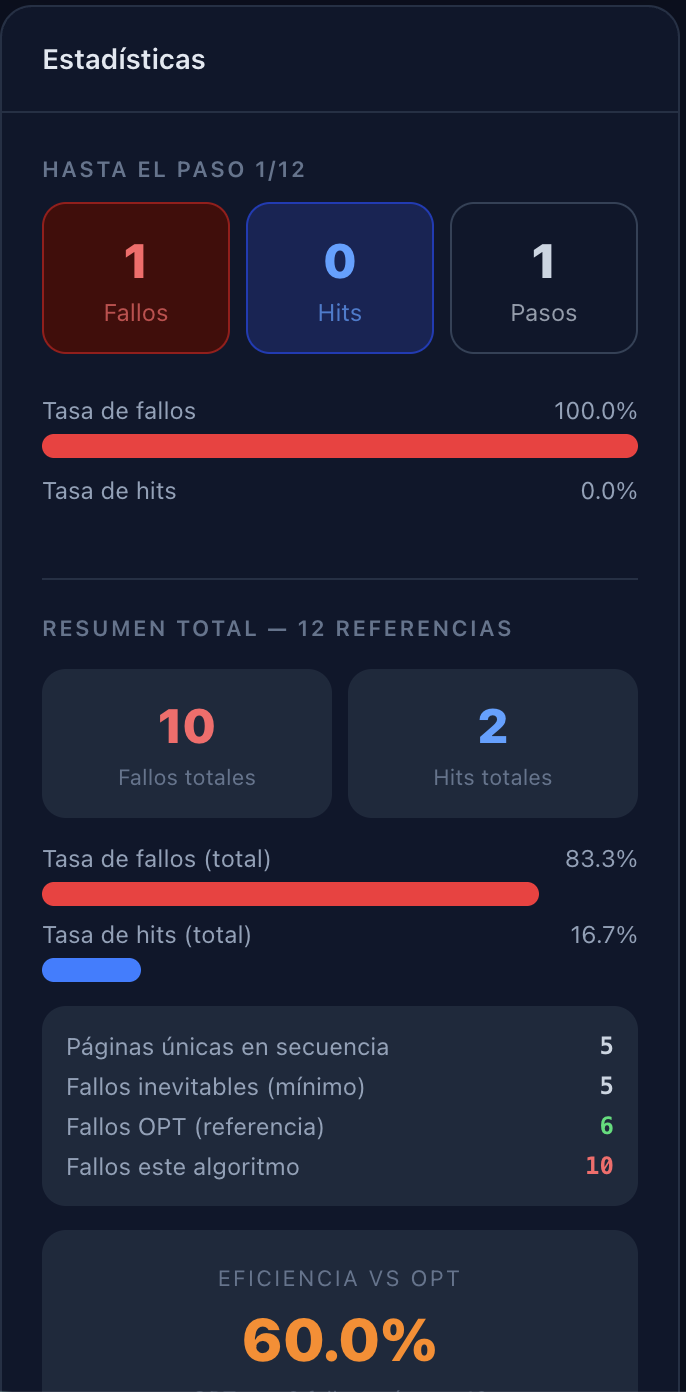
\includegraphics[width=0.48\textwidth]{cap2.png}
  \caption{Panel de estadísticas con FIFO: 10 fallos totales, tasa de fallos 83.3\%, eficiencia vs OPT 60\%.}
  \label{fig:stats}
\end{figure}

\begin{itemize}
  \item Fallos e hits acumulados hasta el paso actual.
  \item Fallos e hits totales de la simulación completa.
  \item \textbf{Fallos inevitables}: las primeras \(n\) páginas únicas (mínimo absoluto).
  \item \textbf{Fallos OPT}: resultado de ejecutar OPT con la misma configuración (referencia teórica).
  \item \textbf{Eficiencia vs OPT}:
  \[
    \text{Eficiencia} = \frac{\text{Fallos OPT}}{\text{Fallos algoritmo}} \times 100\%
  \]
\end{itemize}

% ─────────────────────────────────────────────────────────────────────────────
\section{Panel de Métricas}
% ─────────────────────────────────────────────────────────────────────────────

Tras ejecutar la simulación, el panel de métricas presenta cuatro secciones:

\begin{figure}[H]
  \centering
  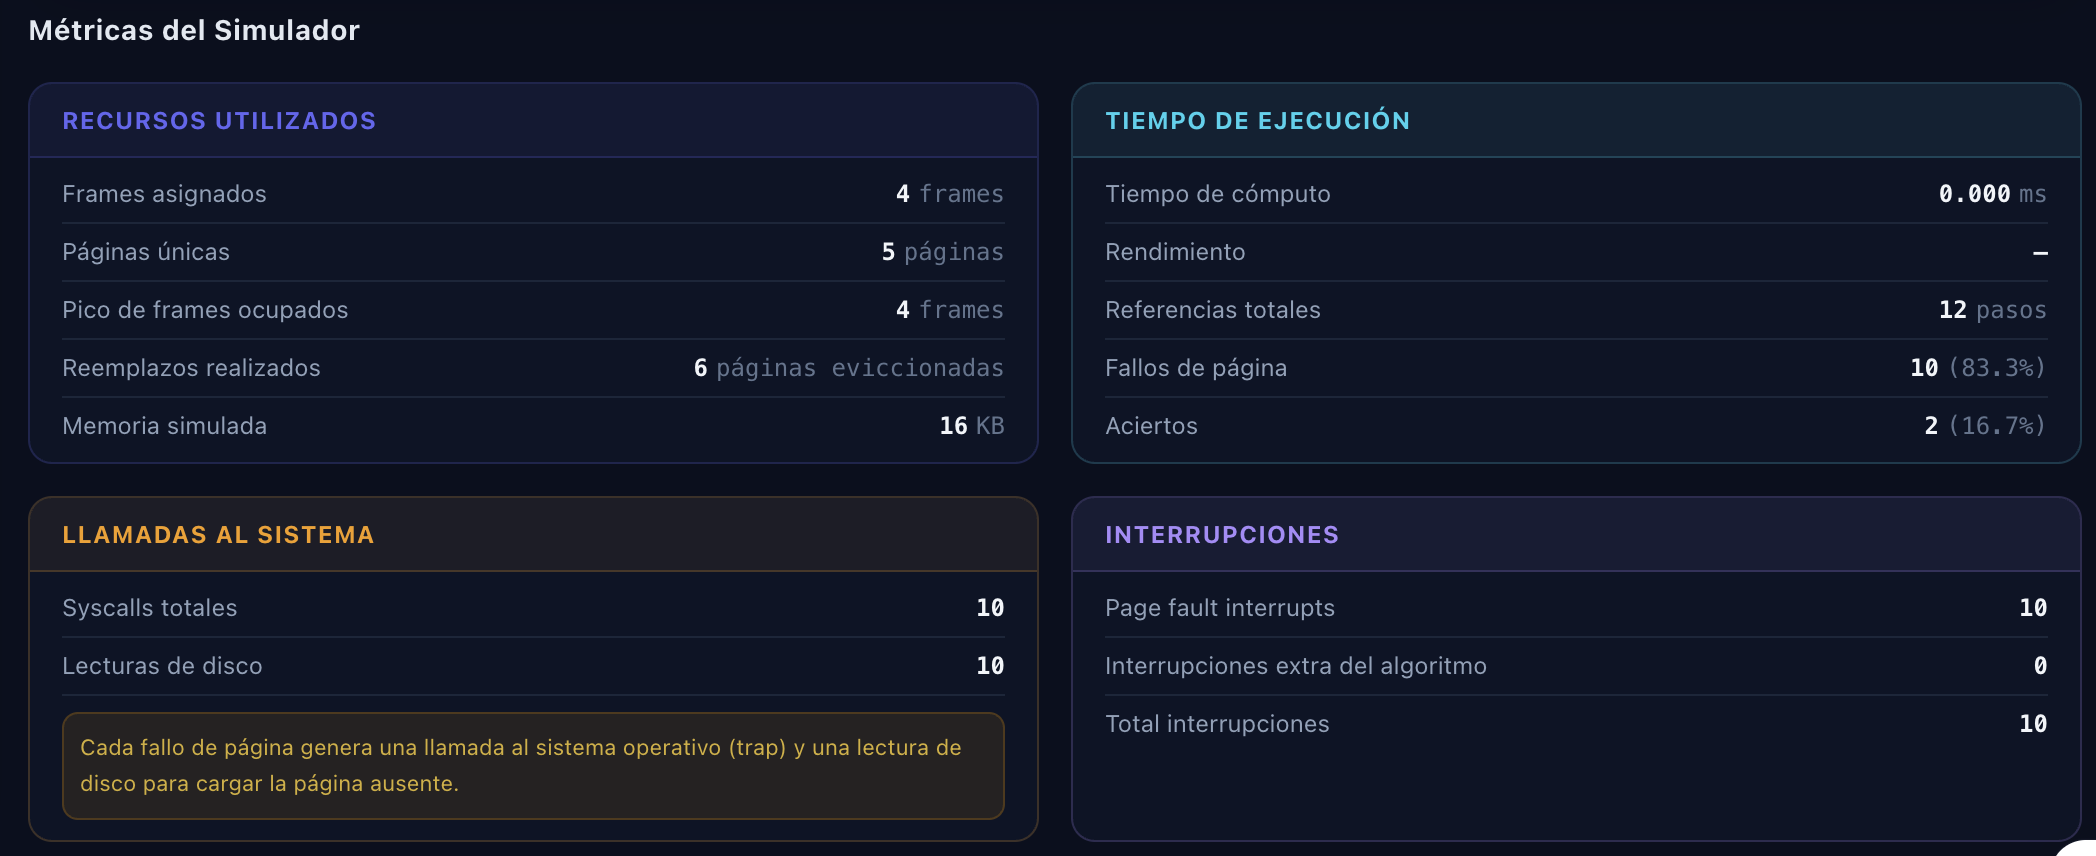
\includegraphics[width=\textwidth]{cap5.png}
  \caption{Panel de métricas con FIFO — 4 marcos, secuencia de 12 referencias. Se muestran las 4 secciones: recursos, tiempo de ejecución, llamadas al sistema e interrupciones.}
  \label{fig:metricas}
\end{figure}

\subsection{Recursos Utilizados}

\begin{itemize}
  \item \textbf{Frames asignados}: número de marcos configurados.
  \item \textbf{Páginas únicas}: cardinalidad del conjunto de páginas referenciadas.
  \item \textbf{Pico de frames ocupados}: máximo de frames en uso simultáneo.
  \item \textbf{Reemplazos realizados}: fallos con frame lleno (evictions reales).
  \item \textbf{Memoria simulada}: \(\text{frames} \times 4\,\text{KB}\).
\end{itemize}

\subsection{Tiempo de Ejecución}

\begin{itemize}
  \item \textbf{Tiempo de cómputo}: milisegundos reales medidos con \texttt{performance.now()}.
  \item \textbf{Rendimiento}: referencias procesadas por milisegundo.
  \item Fallos y hits con su porcentaje.
\end{itemize}

\subsection{Llamadas al Sistema}

Cada fallo de página genera:
\begin{itemize}
  \item \textbf{1 syscall} (la excepción/trap al SO).
  \item \textbf{1 lectura de disco} (para traer la página ausente).
\end{itemize}

Por tanto: \(\text{Syscalls totales} = \text{Lecturas de disco} = \text{Total fallos}\).

\subsection{Interrupciones}

\begin{itemize}
  \item \textbf{Page fault interrupts}: una por cada fallo (\(= \text{total fallos}\)).
  \item \textbf{Interrupciones extra por algoritmo}:
    \begin{itemize}
      \item \textbf{CLOCK}: suma de \texttt{stepsToReplace} en todos los fallos (pasos del puntero buscando víctima).
      \item \textbf{NRU}: valor final de \texttt{tickCount} (número de resets del bit R).
      \item Resto de algoritmos: 0.
    \end{itemize}
  \item \textbf{Total interrupciones}: suma de las dos anteriores.
\end{itemize}

% ─────────────────────────────────────────────────────────────────────────────
\section{Análisis Comparativo de Algoritmos}
% ─────────────────────────────────────────────────────────────────────────────

\subsection{Secuencia de Prueba}

Se emplea la secuencia clásica de Bélady:
\[
  1,\; 2,\; 3,\; 4,\; 1,\; 2,\; 5,\; 1,\; 2,\; 3,\; 4,\; 5
\]
con \textbf{4 marcos} y \textbf{12 referencias}.

\subsection{Resultados}

\begin{center}
\begin{tabular}{lcccc}
  \toprule
  Algoritmo & Fallos & Hits & Tasa fallos & Eficiencia vs OPT \\
  \midrule
  OPT   & 6  & 6  & 50.0\% & 100.0\% \\
  LRU   & 8  & 4  & 66.7\% & 75.0\%  \\
  Clock & 8  & 4  & 66.7\% & 75.0\%  \\
  NRU   & 8--10 & 2--4 & 66--83\% & 60--75\% \\
  LFU   & 8  & 4  & 66.7\% & 75.0\%  \\
  FIFO  & 10 & 2  & 83.3\% & 60.0\%  \\
  MFU   & 10 & 2  & 83.3\% & 60.0\%  \\
  \bottomrule
\end{tabular}
\end{center}

\textit{Nota:} NRU varía según los valores del bit~M. El simulador permite modificarlos manualmente para observar el impacto.

\subsection{Observaciones}

\begin{enumerate}
  \item \textbf{OPT} establece el mínimo teórico de 6 fallos. Ningún algoritmo online puede alcanzarlo de forma consistente.
  \item \textbf{LRU y Clock} empatan en esta secuencia con 8 fallos. Clock es preferido en implementaciones reales por su menor costo de mantenimiento.
  \item \textbf{FIFO} produce 10 fallos y demuestra la \textit{Anomalía de Bélady}: con 3 marcos producía 9 fallos, más eficiente que con 4.
  \item \textbf{MFU} también produce 10 fallos, confirmando que la heurística de expulsar la más frecuente es contraproducente en esta carga típica.
  \item \textbf{NRU} es el más impredecible por la dependencia del bit M y el intervalo de reset del bit R.
\end{enumerate}

% ─────────────────────────────────────────────────────────────────────────────
\section{Implementación Destacada}
% ─────────────────────────────────────────────────────────────────────────────

\subsection{Pre-cómputo de Snapshots}

El diseño clave del simulador es que \textbf{todos los pasos se calculan de una vez} al ejecutar. Esto permite:
\begin{itemize}
  \item Navegar hacia atrás sin necesidad de re-ejecutar el algoritmo.
  \item Calcular las estadísticas totales inmediatamente.
  \item Usar un scrubber para saltar a cualquier paso en $O(1)$.
\end{itemize}

\subsection{NRU con Bit M Editable}

El algoritmo NRU acepta un parámetro \texttt{dirtyOverrides: Record<number, boolean>} que mapea índices de paso a valores de bit M. Al hacer clic en un badge en la tabla, el simulador:
\begin{enumerate}
  \item Registra el override en el estado global.
  \item Re-ejecuta \textbf{toda} la simulación con los overrides actualizados.
  \item El panel se actualiza al instante.
\end{enumerate}

\subsection{Medición de Tiempo y Métricas}

Las métricas de tiempo usan la API \texttt{performance.now()} del navegador, que ofrece resolución de microsegundos:

\begin{lstlisting}[language=JavaScript, caption={Medición de tiempo de cómputo en el reducer}]
case 'RUN_SIMULATION': {
  const t0 = performance.now();
  const snapshots = computeSnapshots(
    state.algorithm, state.pageSequence,
    state.frameCount, state.dirtyOverrides
  );
  const executionTimeMs = performance.now() - t0;
  const metrics = computeMetrics(
    snapshots, state.algorithm,
    state.frameCount, executionTimeMs
  );
  return { ...state, snapshots, metrics,
           currentStep: 0, isConfigured: true };
}
\end{lstlisting}

\subsection{Cálculo de Interrupciones Extra}

La función \texttt{computeMetrics} extrae las interrupciones extra según el algoritmo:

\begin{lstlisting}[language=JavaScript, caption={Cálculo de interrupciones extra por algoritmo}]
if (algorithm === 'CLOCK') {
  extraInterrupts = snapshots
    .filter(s => s.isFault)
    .reduce((sum, s) => sum + s.variables.stepsToReplace, 0);
} else if (algorithm === 'NRU') {
  const lastSnap = snapshots[snapshots.length - 1];
  extraInterrupts = lastSnap.variables.tickCount;
}
\end{lstlisting}

% ─────────────────────────────────────────────────────────────────────────────
\section{Conclusiones}
% ─────────────────────────────────────────────────────────────────────────────

\begin{enumerate}
  \item Se implementó exitosamente un simulador interactivo que cubre los siete algoritmos de reemplazo de páginas más importantes del temario de Sistemas Operativos: FIFO, LRU, NRU, OPT, Clock, LFU y MFU.

  \item El diseño basado en \textbf{pre-cómputo de snapshots} demuestra ser una arquitectura eficiente para simuladores pedagógicos: permite navegación bidireccional libre y cálculo inmediato de estadísticas globales.

  \item Los resultados con la secuencia clásica confirman las predicciones teóricas: OPT es el óptimo inalcanzable, LRU y Clock son las mejores aproximaciones prácticas, FIFO exhibe la Anomalía de Bélady y MFU se desempeña pobremente en cargas generales.

  \item El panel de métricas añade valor pedagógico al relacionar los conceptos de algoritmos con las consecuencias a nivel de SO: cada fallo de página implica una llamada al sistema y una lectura de disco, lo que justifica el esfuerzo en diseñar algoritmos de reemplazo eficientes.

  \item La posibilidad de editar el bit~M en NRU en tiempo real permite al estudiante experimentar cómo la distinción entre páginas limpias y sucias afecta las decisiones de reemplazo.

  \item El proyecto demuestra la sinergia entre herramientas modernas de desarrollo web (React, TypeScript, Tailwind) y el desarrollo de herramientas educativas de sistemas de bajo nivel.
\end{enumerate}

% ─────────────────────────────────────────────────────────────────────────────
\section*{Referencias}
% ─────────────────────────────────────────────────────────────────────────────
\addcontentsline{toc}{section}{Referencias}

\begin{enumerate}[label={[\arabic*]}]
  \item Tanenbaum, A. S., \& Bos, H. (2015). \textit{Modern Operating Systems} (4th ed.). Pearson.
  \item Silberschatz, A., Galvin, P. B., \& Gagne, G. (2018). \textit{Operating System Concepts} (10th ed.). Wiley.
  \item Bélady, L. A. (1966). A study of replacement algorithms for a virtual-storage computer. \textit{IBM Systems Journal}, 5(2), 78--101.
  \item Repositorio del proyecto: \url{https://github.com/hectorDev2/algoritmos-paginacion-so}
\end{enumerate}

\end{document}
